% !TeX encoding = UTF-8

% 载入 SJTUThesis 模版
\documentclass[type=master]{sjtuthesis}
% 选项
%   type=[doctor|master|bachelor|course],     % 可选(默认:doctor),论文类型
%   zihao=[-4|5],                             % 可选(研究生默认:-4,本科默认:5),正文字号大小
%   language=[chinese|english],               % 可选(默认:chinese),论文的主要语言
%   review,                                   % 可选(默认:关闭),盲审模式
%   [twoside|oneside]                         % 可选(默认:twoside),单双页模式

% 论文基本配置,加载宏包等全局配置
% !TEX root = ./main.tex

\sjtusetup{
  %
  %******************************
  % 注意:
  %   1. 配置里面不要出现空行
  %   2. 不需要的配置信息可以删除
  %******************************
  %
  % 信息录入
  %
  info = {%
    %
    % 标题
    %   可使用“\\”命令手动控制换行
    %
    title           = {CIS片内神经网络算法推理模块的建模},
    title*          = {Modeling of Inference for CIS On-Chip Neural Network Algorithm},
    %
    % 关键词
    %
    keywords        = {建模, CMOS图像传感器, 神经网络},
    keywords*       = {Model, CIS, Neural Network},
    %
    % 姓名
    %
    author          = {龚\quad{}烽},
    author*         = {Gong Feng},
    %
    % 指导教师
    %
    supervisor      = {张忠能教授},
    supervisor*     = {Prof. Zhang Zhongneng},
    %
    % 副指导教师
    %
    % assisupervisor  = {某某教授},
    % assisupervisor* = {Prof. Uom Uom},
    %
    % 学号
    %
    id              = {116033210009},
    %
    % 学位
    %   本科生不需要填写
    %
    degree          = {工学硕士},
    degree*         = {Master of Engineering},
    %
    % 专业
    %
    major           = {计算机技术},
    major*          = {Computer Technology},
    %
    % 所属院系
    %
    department      = {电子信息与电气工程学院},
    department*     = {School of Electronic Information and Electrical Engineering},
    %
    % 课程名称
    %   仅课程论文适用
    %
    %course          = {某某课程},
    %
    % 答辩日期
    %   使用 ISO 格式 (yyyy-mm-dd);默认为当前时间
    %
    % date            = {2014-12-17},
    %
    % 资助基金
    %
    % fund  = {
    %           {国家 973 项目 (No. 2025CB000000)},
    %           {国家自然科学基金 (No. 81120250000)},
    %         },
    % fund* = {
    %           {National Basic Research Program of China (Grant No. 2025CB000000)},
    %           {National Natural Science Foundation of China (Grant No. 81120250000)},
    %         },
  },
  %
  % 风格设置
  %
  style = {%
    %
    % 本科论文页眉 logo 颜色
    %   默认为黑色
    %
    % header-logo-color = red,
  },
  %
  % 名称设置
  %
  name = {%
    % publications      = {攻读学位期间完成的论文},
  },
}

% 参考文献支持宏包
\usepackage[backend=biber,style=gb7714-2015,gbnamefmt=lowercase,gbpub=false,gbpunctin=false]{biblatex}
% 导入参考文献数据库
\addbibresource{bibdata/thesis.bib}

% 定义图片文件目录与扩展名
\graphicspath{{figures/}}
\DeclareGraphicsExtensions{.pdf,.eps,.png,.jpg,.jpeg}

% 确定浮动对象的位置,可以使用 [H],强制将浮动对象放到这里(可能效果很差)
% \usepackage{float}

% 固定宽度的表格
% \usepackage{tabularx}

% 表格中支持跨行
\usepackage{multirow}

% 表格中数字按小数点对齐
\usepackage{dcolumn}
\newcolumntype{d}[1]{D{.}{.}{#1}}

% 使用长表格
\usepackage{longtable}

% 附带脚注的表格
\usepackage{threeparttable}

% 算法环境宏包
\usepackage[ruled,vlined,linesnumbered]{algorithm2e}
% \usepackage{algorithm}

% 代码环境宏包
\usepackage{listings}
\lstnewenvironment{codeblock}[1][]
  {\lstset{style=lstStyleCode,#1}}{}

% 国际单位制宏包
\usepackage{siunitx}

% 定理环境宏包
\usepackage{ntheorem}
% \usepackage{amsthm}

% 绘图宏包
\usepackage{tikz}

% 一些文档中用到的 logo
\usepackage{hologo}
\newcommand{\XeTeX}{\hologo{XeTeX}}
\newcommand{\BibLaTeX}{\textsc{Bib}\LaTeX}

% 借用 ltxdoc 里面的几个命令方便写文档
\DeclareRobustCommand\cs[1]{\texttt{\char`\\#1}}
\providecommand\pkg[1]{{\sffamily#1}}

% 自定义命令

% E-mail
\newcommand{\email}[1]{\href{mailto:#1}{\texttt{#1}}}

% hyperref 宏包在最后调用
\usepackage{hyperref}


\begin{document}

%TC:ignore

% 无编号内容

% 论文标题页
\maketitle

% 原创性声明、版权授权页
\originalitypage*
\copyrightpage[scans/copyright.pdf]

% 使用罗马数字对前文编号
\frontmatter

% 摘要
% !TEX root = ../main.tex

\begin{abstract}
  本文内容是一种在CMOS图像传感器(CIS)的片内进行深度学习图像推理运算的专用SoC的建模和仿效。
  这种在CIS芯片片内进行深度学习神经网络推理的方案与传统的CPU、GPU等通用GPP对CSI-TX接口输出的视频流进行推理的做法相比,在存储性能和计算性能上具有优势。
  与业内常见的专用深度学习加速芯片相比,在CIS片内的设计能够带来带宽上的优势,同时也可以利用片内数据通路的流水线特性,设计专用的并行算法来提高运算速度。
  另外一方面,随着当今集成电路领域的发展,芯片设计的规模变得越来越庞大。
  电路的性能已经得到极大的提高,单个芯片上的晶体管数达亿级甚至十亿级,使得更多的模块能够集成到一个芯片上。
  但随着集成电路的规模变大,设计和验证的工作也变得更加繁重。
  为了提高项目的质量,提早验证系统和算法的设计,对芯片进行系统级和算法级建模和验证变得非常重要。这也是本文中工作的意义所在。


\end{abstract}

\begin{abstract*}
  The content of this paper is the modeling and imitation of a special SOC for deep learning image reasoning operation in the chip of CMOS image sensor (CIS).
  This scheme of deep learning neural network reasoning in cis chip has advantages in storage performance and computing performance compared with the traditional method of reasoning the video stream output by csi-tx interface by general GPPS such as CPU and GPU. Compared with the common dedicated deep learning acceleration chip in the industry, the design in cis chip can bring the advantage of bandwidth. At the same time, it can also use the pipeline characteristics of on-chip data path to design a dedicated parallel algorithm to improve the operation speed.  

  On the other hand, with the development of today's integrated circuit field, the scale of chip design becomes larger and larger. The performance of the circuit has been greatly improved. The number of transistors on a single chip has reached hundreds of millions or even billions, so that more modules can be integrated into one chip.
  However, as the scale of integrated circuits becomes larger, the work of design and verification becomes more and more arduous. In order to improve the quality of the project and verify the design of system and algorithm in advance, it is very important to model and verify the chip at system level and algorithm level. This is also the significance of the work in this paper.
\end{abstract*}


% 目录、插图索引、表格索引、算法索引
\tableofcontents
\listoffigures*
\listoftables*
\listofalgorithms*

% 主要符号对照表
% !TEX root = ../main.tex

\begin{nomenclature*}
\label{chap:symb}

\begin{longtable}{rl}
  $\gamma$    & 缩放系数  \\
  $\beta$     & 位移系数  \\
  $eps$       & 数值稳定性常数  \\
  $\mu$       & 均值      \\
  $\sigma$    & 方差      \\
  

\end{longtable}

\end{nomenclature*}


%TC:endignore

% 使用阿拉伯数字对正文编号
\mainmatter

% 正文内容
% !TEX root = ../main.tex

\chapter{课题背景和研究意义}

本章节将介绍CIS芯片的前端设计和深度学习网络软硬件发展的背景,讨论两者之间的联系以及
研究的内容和意义。

\section{国内外研究现状}
本章节将从描述CIS芯片开始,结合人工智能软硬间发展的历史,引出本课题的背景研究意义。


\subsection{ASIC与CIS芯片}
%TODO 描述ASIC的基本概念
%TODO 描述CIS芯片的基本概念
CMOS Image Sensor(CIS)就是一种基于CMOS工艺制造的图像传感器。
我们现今常见的照相机、安防摄像头、手机摄像头内使用的图像传感器大多都是采用的CIS芯片。
CIS芯片也属于一种专用集成电路(ASIC)。
专用集成电路(ASIC)的全称是Application Specific Integrated Circuit,它是一种用于特定场景或者用途的芯片。
ASIC设计对任何公司来说都是一项高难度的挑战。  

近年,CIS芯片市场供不应求,技术飞速发展。CMOS图像传感器是一种典型的固体成像传感器,与CCD有着共同的历史渊源。
CMOS图像传感器通常由像敏单元阵列、行驱动器、列驱动器、时序控制逻辑、AD转换器、数据总线输出接口、控制接口等几部分组成, 这几部分通常都被集成在同一块硅片上。
其工作过程一般可分为复位、光电转换、积分、读出几部分。  
索尼在2012年推出了全球首款用于消费电子产品的堆叠芯片CIS相机系统(CIS+ISP)。
在2017年的ISSCC大会上,索尼又发布了他们的一款三层堆栈式CIS\parencite{sony2017}。 %引用 
其结构为:顶层的图像感知层、中间的DRAM层和底层的逻辑电路层(CIS+DRAM+ISP)。
堆栈式CIS芯片成为了发展趋势。
随着各厂商的设计能力与工艺的提升,越来越多的IP被集成到CIS芯片的堆栈中,使得现今的CIS芯片功能更加强大和复杂。
由于堆栈式设计的存在,使得我们将深度学习神经网络的运算模块叠加在CIS芯片中成为可能。  

\subsection{深度学习和残差网络}
想要实现深度学习神经网络算法的硬件加速,就先要对深度学习神经网络算法有所了解。
% 简述DL的发展,例举出最经典的一些算法。
卷积神经网络(Convolutional Neural Networks, CNNs)\parencite{cnn1998}和深度神经网络(Deep Neural Networks, DNNs)\cite{dl2015}是目前最先进的两种机器学习算法之一。
%引用 Y. LeCun, L. Bottou, Y. Bengio, and P. Haffner, “Gradient-Based Learning Applied to Document Recognition,” Proceedings of the IEEE, vol. 86, no. 11, pp. 2278– 2324, 1998.
%引用 Deep Learning, by Yann L., Yoshua B. & Geoffrey H. (2015) 
它们都属于多层感知器(MLPs)家族,可能包括四种类型的层:卷积层、池化层、归一化层和分类器层\parencite{NN1998}。%引用
%引用  S. Haykin, Neural Networks: A Comprehensive Foundation, 2nd ed. Upper Saddle River, NJ, USA: Prentice Hall PTR, 1998.
回顾深度学习算法的发展史,始于LeNet识别了10个手写的数字。
它是一种广泛用于文档识别的卷积神经网络,由两个卷积层、两个池层和三个分类器层组成。
卷积层实际上是一种滤波器。它可以用来识别输入的特征图的某些特征。
每个局部滤波器都有一个$K_x$x$K_y$尺寸的核,用来处理卷积窗口。
这个卷积窗口将捕获一个输入特征映射中的$K_x$x$K_y$尺寸的输入神经元。
局部滤波器的2D阵列产生一个输出特征映射。
其中的每一个局部滤波器对应一个输出神经元。
深度学习算法的爆发期在2012年至2017年。
2012年多伦多大学的Geoffrey Hinton的课题组首次参加ImageNet图像识别比赛,就通过其构建的卷积神经网络AlexNet\cite{alexnet2012}一举夺得冠军。
他们的成绩大幅超出了第二名(一种SVM)的分类性能。
这使得AlexNet成为近年的一个里程碑。
%引用 Krizhevsky A, Sutskever I, Hinton G E. Imagenet classification with deep convolutional neural networks[C]//Advances in neural information processing systems. 2012: 1097-1105.


% 简述ResNet
% TODO 简述ResNet18的网络结构
近几年的ImageNet比赛中,网络的深度越来越深。
随着网络的加深,产生了梯度消失或者梯度爆炸的问题,导致训练的准确率下降的现象。
这种现象并不是由过拟合导致的,因为过拟合的现象发生时,训练的准确率会表现得非常高。
针对这个问题何恺明博士在2015年提出的ResNet\parencite{resnet2015}很好地解决了这个问题,并在2015年的ImageNet比赛上获得了第一名。
% 引用
ResNet18由4个主要的残差层组成。
整个网络的开头,由7x7的卷积核做卷积运算和3x3的最大池化。
卷积运算有64个输出的通道。设定的步长是2,填充的边框是3。
最大值池化的步长是2,填充的边框是1。
最后输出的图像尺寸是112x112

之后是四个包含两个BasicBlock来做运算的残差层。
每个BasicBlock中都有两个3x3的卷积运算。
它们的深度不同,分别是64、128、256和512。
ResNet可能使用两种不同的残差单元。一种是BasicBlock,用于ResNet18和ResNet34这种浅层网络。
另一种是Bottleneck,用于50层及以上的ResNet。

% 实现哪一种深度学习算法
本课题中,将要通过设计专用的硬件加速器来进行ResNet18的前向计算。
因此,这一小节将分析ResNet18所涉及到的所有基本运算。


\subsection{深度学习运算的硬件}
现在,市场上有许多可用以深度学习神经网络或卷积神经网络的设备。
常见的,我们会使用GPU来进行网络模型的训练或是图像识别的推理。
这些设备有的在云端,有些在工作站或台式设备上,还有些在移动端甚至在我们身上的可穿戴设备上。
这一章节将介绍深度学习运算硬件的发展史,以及如何评价一种深度学习运算硬件的性能好坏的方法。


\subsubsection{深度学习运算硬件的发展史}

感知时代始于2012年。之后谷歌在几千台普通机器上进行了出色的并行CPU有损更新研究。
在这之后的2014年,VGGNet与GoogLenet相继诞生,专为神经网络设计的硬件在90年代初诞生。
CNAPS(1990),它带有64个处理单元和256kB内存,可以在8/16位条件下达到1.6 GCPS的速度(CPS是指每秒连接次数 / connections per second)或在1位条件下达到12.8GCPS的速度\cite{Heemskerk1995OverviewON}。
%引用   Overview of neural hardware

随着大数据和深度学习的发展,用于相关领域的硬件发展趋势也受到业内人士以及专家们的广泛关注。
在半导体领域,2019 ISSCC大会于2月17—21日在美国旧金山开幕。
Facebook首席AI科学家Yann LeCun在会上发表了主题演讲”深度学习硬件:过去、现在和未来“,详细介绍了深度学习研究的发展将如何影响未来硬件架构\cite{Yann2019DeepLH}。
%引用  ISSCC 2019 Deep Learning Hardware: Past, Present, and Future


深度神经网络在图像的识别、分类、检测和分割等领域起到了非常重要的作用。
在各种DNN的网络结构中,卷积神经网络是最常见的一种。
常见的硬件加速方案中,主要有CPU、GPU、FPGA和ASIC。
如图\ref{fig:silicon_alternatives}所示,这些半导体器件在应用灵活度和能效比两方面的关系成反比。  
\begin{figure}[htbp]
    \centering
    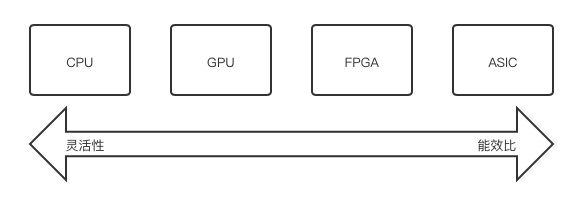
\includegraphics[width=15cm,height=4.5cm]{figures/silicon_alternatives.png}
    \caption{半导体器件能效比与灵活度关系示意图}
    \label{fig:silicon_alternatives}
\end{figure}

CPU和GPU的方案依赖于指令集和编译器的支持。
在实际应用中,GPU无论在训练深度学习神经网络的模型,还是图像识别或分类等深度学习的应用上,都比CPU更具有优势。
GPU相比CPU主要具有以下三点优势:
\begin{enumerate}
    \item 提供了更多可供并行计算的基础计算单元。典型地,这里的并行可以理解为单次执行多条指令的算法。
    \item 防存速度更快,因为GPU的每个核都拥有自己独立的cache;
    \item 一般的,GPU比CPU具有更高的浮点数运算能力。
\end{enumerate}
在常见的CPU和GPU平台上,SIMT和SIMD等技术被广泛地应用。
从字面上解释,SIMT是单指令多线程,而SIMD为单指令多数据流。
在SIMD中,向量中的元素处在相同的地址空间。
而SIMT中的每一个线程的寄存器都是私有的。可以通过共享内存或是其他的线程内同步机制来进行通信。
FPGA是可编程逻辑门电路,这种方案既可以实现算法的硬件加速,又可以不用支付ASIC后端开发和流片的成本。
ASIC作为一种专用的硬件加速方案,在性能和功耗,特别是能耗比上,是其他几种方案都无法相比的。
一般地,这种芯片被称为嵌入式神经网络处理器(NPU)。


\subsubsection{评价硬件的影响因子}
上一节中提到了CPU、GPU、FPGA、ASIC四个类型的半导体器件。
那么如何评价这些硬件在深度学习运算上的表现呢?
这一小节总结了主要的评价硬件在深度学习运算上的影响因子。
它们是精准度、吞吐量、延迟、能效比和功耗。

% TODO 精确度 吞吐量和延迟 能效比和功耗
准确度是这类问题中最常见的一个指标。对于图像分类问题,准确度报告为正确分类图像的百分比,而对于目标检测问题,精度报告为平均准确度。
影响准确性的因素包括任务的难度和数据集。因此,准确度在建模的过程中将被用来验证设计的正确性。
吞吐量用于指示在给定时间段内可以处理的数据量或可以完成的任务的执行次数。高吞吐量通常是应用程序的关键。
延迟度量输入数据到达系统和生成结果之间的时间。低延迟对于实时交互应用程序(如虚拟现实、自主导航和机器人技术)是必要的。
吞吐量和延迟通常被认为是可以直接相互派生的。
一般的,在给定能量单位下可处理的数据量或完成任务的执行次数被称为能效比。


近年,通过FPGA和ASIC实现硬件神经网络加速器的方式在功耗和性能上展现出了巨大的优势。
工程师们还想要进一步降低功耗和提升性能受到存储器访问的限制。
本课题关注的是图像识别的应用。用于该应用的最先进的神经网络算法就是卷积神经网络,它的一个重要特性就是权重在神经元之间共享。
这种特性大幅减少了在神经网络的运算中所使用的内存,允许我们在SRAM中完全映射一个卷积神经网络,并且避免访问DRAM来读取权重值。
而CIS芯片的数据通路具有流水线的特性,使得这种设计具有通用的深度学习加速器不具有的并行运算能力。
另外,加速器本身处在数据通路中,将会进一步减少为了读取输入数据和写入输出数据而进行的DRAM访问。   

与机器学习或深度学习相关的边缘计算领域也在今年得到了长足的发展。
例如:由Pete Warden 与 Daniel Situnayake在2019年提出的TinyML就是在毫瓦功率的微处理器上,实现机器学习算法、工具和技术\cite{tinyml2019}。
%引用  TinyML
这一技术是基于Tensorflow Lite在微控器上的软件框架和硬件环境而来的。
一般来说,它只需要几十千字节的存储空间。  

在CIS的领域,物联网中的感知节点数量持续快速增长,产生海量数据。
到2032年,从感官节点产生的信息相当于1020bit/s,远大于人类感官总吞吐量\cite{2020Near}。
%引用  Near-Sensor and In-Sensor Computing
尽管5G网络或是将来的6G网络会为物联网提供高速传输和大带宽。
因此,近传感器和传感器内计算范式的概念被提了出来。
通过它们在传感器和运算单元之间的位置来定义它们输入哪一种类型。
因为感知功能是在有噪声的模拟域中实现的,使用集成在同一域中的模拟处理器来处理传感器数据是非常理想的,这种类型就是传感器内计算。
这种高效率运算系统避免了数模转换,减少了延迟和功耗。


\subsection{ShiDianNao与谷歌TPU}
近几年,市场上的NPU百花齐放。
几乎所有市场上旗舰手机的SoC都嵌入了NPU。
由于各家厂商嵌入在SoC中的NPU各不相同,因此性能和功耗也是天差地别。
各个厂家也是对这个新ip讳莫如深。
公开可查到的有谷歌TPU\cite{2017In}和寒武纪的Diannao\cite{2014DianNao}系列。
它们的设计思想可以作为后续设计的参考。
当前情况下,寒武纪的Diannao系列显得比谷歌的TPU更开放一些。
寒武纪开放了其指令集Cambricon\cite{2016Cambricon}和相应的工具链或者是云服务。
同时,寒武纪的Diannao系列作品的论文也非常完整,特别是ShiDianNao\cite{2015ShiDianNao}对本课题有非常大的借鉴意义。
谷歌TPU方面,我们只能通过Google Colab服务来使用云端的TPUs。
在最新款的谷歌手机上,名为Google Tensor的SoC芯片内置了Google edge TPU来加强机器学习的运算能力。
但谷歌没有开放相关的SDK,因此可以相信这个TPU只是给设备原生的一些应用使用的。


\subsubsection{ShiDianNao和边缘计算}
%TODO 简单介绍shidiannao和Cambricon的原理
在国内,寒武纪的DianNao系列产品可谓是深度学习处理器的先驱。
DianNao是在2014年寒武纪深度学习处理器的开山之作。
它可以被看作是此系列处理器的硬件设计基础。
后来的的DaDianNao、ShiDianNao、PuDianNao则分别适用于服务器端的高性能计算、设备端边缘计算和更加泛化的机器学习算法。
其中,DianNao、DaDianNao和PuDianNao采用了流水线式乘加树的结构。  %引用   


% ShiDianNao的整体架构描述。
% ShiDianNao的整体架构贴图。
% ShiDianNao的DL加速单元架构描述。
% 上述架构的贴图
ShiDianNao是一个放置在CMOS或CCD传感器旁的CNN加速器\cite{2015ShiDianNao}。
它有特定的数据访问模式来避免DRAM的读写访问。
这是的ShiDianNao具有以前最先进的神经网络加速器的60倍的能效比。
它在65纳米的布局下,面积为4.86 $mm^2$,功耗仅为320 mW,但仍然比高端GPU快30倍。

\begin{figure}[htbp]
    \centering
    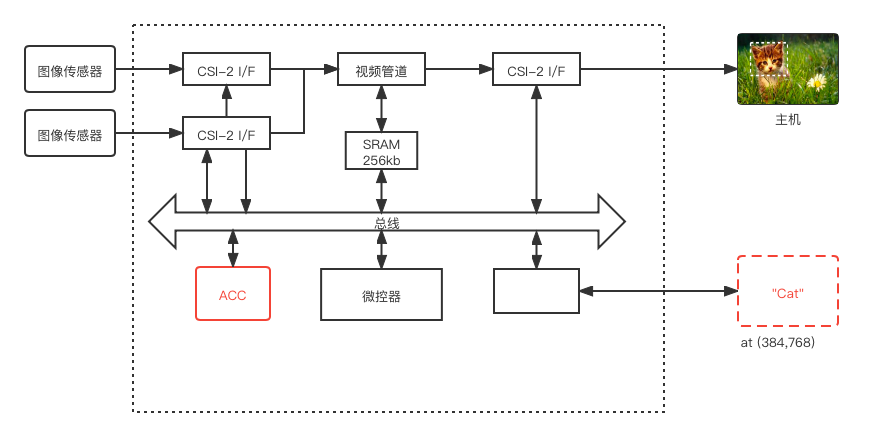
\includegraphics[width=15cm,height=8cm]{figures/ShiDianNao_arch.png}
    \caption{ShiDianNao的架构图}
    \label{fig:shidiannao_arch}
\end{figure}
ShiDianNao的架构设计如图\ref{fig:shidiannao_arch}所示\cite{2015ShiDianNao},在整个SoC上类似于一个挂载在总线上的外设。
加速器有两个功能单元,一个NFU用于调节基本神经元操作(乘法、加法和比较),另一个ALU用于执行激活函数计算。
它的核心模块是NFU(神经功能单元)。
NFU是由$P_x$×$P_y$个处理元素(PE)组成的2D网络。
与DianNao系列的其他产品相比,NFU天然地适合2D特征图的拓扑结构。  
神经元(PE)映射的直观方法是将一块$K_x$×$K_y$ PEs($K_x$×$K_y$是内核大小)分配给单个输出神经元,同时计算所有突触。
但是ShiDianNao中,优化了计算方法。
它将每个输出神经元映射到单个PE,并在连接到同一输出神经元的输入神经元(即突触)之间共享每个PE。  
NFU不能覆盖CNN中的所有计算原语,因此ShiDianNao需要一个轻量级ALU来补充PEs。
ALU实现了16位定点算术运算符,包括除法(用于平均池化和归一化层)和非线性激活函数,如tanh()和sigmoid()(用于卷积层和池化层)。


\paragraph{存储与运算}
%TODO 关于存储Multiple Bank的设计(状态机)
% 11/24 这一段需要重写
在设计嵌入式的深度学习加速器时,无论是系统级使用的存储或者是模块中的缓冲,都要选择合适的存储介质。
在片内运算时所使用的存储,都要选择SRAM,而需要大量存储的静态数据可以放在DRAM中。
一般的,SRAM的读写速度和功耗,都远小于DRAM。
但是SRAM的成本很高。下面是一些比较现今的新型存储。  

除了存储介质的不同外,还可以根据存储与运算的架构设计分类,来区分不同的存储类型。
以这种方式,主要可以分为以下三类:
\begin{enumerate}
    \item 近存运算
    \item 存内运算
    \item 传感器内运算
\end{enumerate}   


\subparagraph{近存运算}


先进的存储技术可以降低高密度存储器(如DRAM)的访问能量。
例如,嵌入式DRAM(eDRAM)\cite{2001Embedded}在芯片上提供高密度存储器,以避免关闭芯片电容的高能耗成本;eDRAM的密度比SRAM高2.85倍,能效比DRAM高321倍(DDR3)\cite{2017Efficient}。
与DRAM相比,eDRAM还提供了更高的带宽和更低的延迟。在DNN处理中,eDRAM可用于在芯片上存储数十兆字节的权重和激活,以避免芯片外访问,如DaDianNao\cite{2015DaDianNao}所示。
eDRAM的缺点是其密度低于片外DRAM,并且会增加芯片成本。
DRAM也可以使用硅通孔(TSV)\cite{2018The}堆叠在芯片顶部,而不是将DRAM集成到芯片本身。
这项技术通常被称为三维存储器,并已以混合存储立方体(HMC)\cite{2012Hybrid}和高带宽存储器(HBM)\cite{HBMDRAM}的形式商业化。
3-D内存提供了一个数量级的更高带宽,并且相对于现有的2-D DRAM,访问能量减少了5倍,因为TSV的电容低于典型的片外互连\cite{2017Efficient}。

\subparagraph{存内运算}
% 这段重写
存内处理与传统架构之间有很大的差异。
DNN处理可以使用矩阵向量乘法执行,
对于传统架构,输入激活向量和权重矩阵都从各自的存储器中读出,并由乘累加阵列处理。
一次可以读取的权重数量受内存接口的限制(例如,读取逻辑和内存端口的数量)。
权重的有限内存带宽也可以限制可并行执行的乘加运算操作的数量(即每个周期的操作),从而限制总吞吐量。
存内运算的架构是将计算移动到存储权重矩阵的内存中进行的;
这可以通过避免读取权重矩阵的成本来帮助减少权重的数据移动;
只从内存中读取计算结果,如部分和或最终输出激活,而不是读取权重;
此外,存内运算架构中的处理还可以增加内存带宽,因为可以并行访问的权重数量不再受内存接口的限制;
理论上,整个权重矩阵可以并行读取和处理\cite{2017Efficient}。  

%这段减少,另加入SRAM和DRAM的存内运算内容
有一种叫做非易失性电阻存储器的存储介质,非常适合做存内运算。
将乘累加运算直接集成到高级非易失性高密度存储器中,并将其用作可编程电阻元件。我们称这种元件为忆阻器\cite{IEEE1971L}。
这种方法的优点包括:由于计算被嵌入内存中,从而减少了数据移动,因此降低了能耗;由于内存和计算可以以与DRAM类似的密度进行密集封装,因此增加了密度[106]。
非易失性电阻存储器器件有几种常见的候选器件,包括相变存储器(PCM)、电阻RAM(RRAM或ReRAM)、导电桥RAM(CBRAM)和自旋转移转矩磁RAM(STT-MRAM)[107]。
这些设备在耐久性(即可以写入多少次)、保留时间、写入电流、密度(即单元大小)、变化和速度方面有不同的权衡。
如[108]所述,使用非易失性电阻存储器进行处理有几个缺点。
首先,它受到前面描述的模拟处理的精度降低和ADC/DAC开销的影响。
第二,阵列尺寸受到连接电阻器件的导线的限制;具体而言,对于大型阵列(例如1k×1k),导线能量占主导地位,并且沿导线的红外压降会降低读取精度。
第三,对电阻器件进行编程的写入能量可能非常昂贵,在某些情况下需要多个脉冲。
最后,电阻器件还可能受到器件间和周期间变化的影响,在整个电导范围内具有非线性电导。


\subparagraph{传感器内运算}
%这段新增


\subsubsection{谷歌TPU的脉动阵列}
%TODO 简单介绍谷歌TPU的脉动阵列原理。
% TPU的架构设计描述
% TPU的架构设计图
如图,主机通过PCIe总线发送TPU指令到指令缓冲区。其内部模块通过256位宽的数据通路连接。
谷歌TPU的核心部件是图中右侧的矩阵乘法单元。
它包括了256x256个乘加器,可以执行8位无符号和有符号整数乘法和加法。
在计算得到16位无符号或有符号整数后,保存在32位累加器中。
TPU在运算时的核心思想是利用脉动阵列来减少缓冲区和SRAM的读写访问。
它的理念是保持矩阵乘加单元一直工作。
TPU拥有4级流水线。同时设计了一组指令来控制访存和运算。其中每条指令在单独的阶段执行,主要的指令如下:
\begin{enumerate}
    \item Read\_Host\_Memory
    \item Read\_Weights
    \item MatrixMultiply/Convolve
    \item Activation
    \item Write\_Host\_Memory
\end{enumerate}
设计遵循了解耦访问和执行的原则。
因此在发出Read\_Weights指令之后,MatrixMultiply指令就可以开始执行,不需要等待Read\_Weights指令完成。
如果Read\_Weights/Activation没有准备好,矩阵乘法单元就会停止。

\paragraph{脉动阵列}
脉动阵列\cite{1978Systolic}是1978年KUNG H T提出的一种应用在片上多处理器的体系结构。
它是由多个相同的、结构简单的计算单元以网状形式连接而成的,具有并行性、规律性和局部通信的特征。
%REF KUNG H T, Leiserson C E. Systolic arrays(for VLSI)[C]. Sparse Matrix Proceedings 1978, Society for Industrial and Applied Mathematics, 1979.
脉动一词来源于心血管。
在冯诺依曼的计算机体系中,指令和数据是一起存储在存储器中。
在运算的过程中,数据从存储器中被取出,经过处理器的处理后再写回到存储器中。
这个过程就像是人体的血液循环一样,因此得名脉动。  
\begin{figure}[htbp]
    \centering
    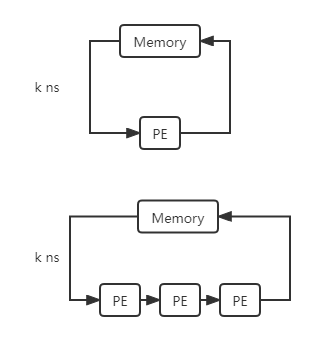
\includegraphics[]{figures/systolic_array.png}
    \caption{脉动阵列原理图}
    \label{systolic}
\end{figure}   

当运算的过程是由多个可重复的运算单元组成时,每一个运算单元都会与一个或者多个周围的单元发生数据交互,结果或将存储在运算单元内部,或将传递给下一个单元。
在脉动阵列中,最重要的是设计一种在运算单元之间联系的规则,并且把高层次的算法映射到每一个单元上。
这里的脉动阵列是使用乘累加器作为其处理单元的。
它非常适合用于如矩阵运算,卷积等等数据流具有一定规律的算法。  

\paragraph{脉动阵列上的卷积运算}
上面两个小节已经分别描述了谷歌TPU\cite{2017In}的架构和普通的脉动阵列做乘加运算的过程。
但是在本课题中需要做的是卷积运算,与矩阵的乘加运算是有区别的。
这一小节将描述谷歌TPU是如何基于脉动阵列执行卷积运算的。
谷歌TPU\cite{2017In}在进行卷积运算时,会把卷积运算转化为二维矩阵乘法。
神经网络处理器会把激活输入和权重输入放到矩阵的行和列中。
激活值和权重在脉动阵列中向右和向下传播(从矩阵左边和上边输入),直到到达指定的运算单元的指定寄存器中。
一旦运算单元中的输入数据都放好,通过控制信号,处理器就会将输入数据经过计算得到输出数据。
这里举一个在谷歌TPU中5x5的激活输入使用3x3的卷积核做卷积的例子,这个输入是170x170大小原图的一部分\cite{2017Rotating}。
如图\ref{fig:activation_and_kernel}是输入的激活和卷积核。
\begin{figure}[htbp]
    \centering
    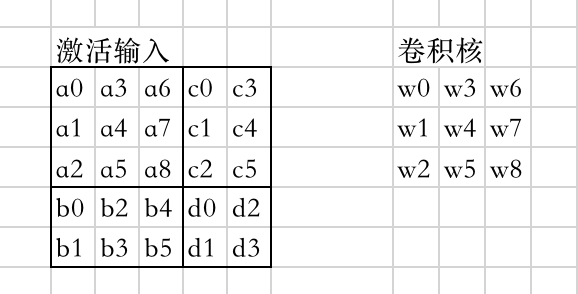
\includegraphics[]{figures/activation_and_kernel.png}
    \caption{输入和卷积核}
    \label{fig:activation_and_kernel}
\end{figure} 

在处理器把激活数据矩阵送进脉动阵列前,会先把矩阵重组为二维的矩阵,然后放入一个向量队列中,然后由多路复用器通过某种算法输入激活。
向量输入队列的排序如图\ref{fig:vector_inputs}所示.
\begin{figure}[htbp]
    \centering
    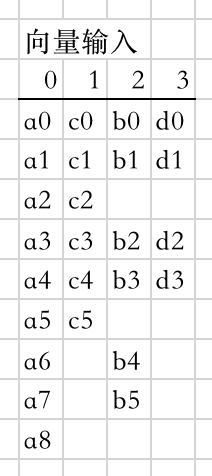
\includegraphics[]{figures/vector_inputs.png}
    \caption{输入和卷积核}
    \label{fig:vector_inputs}
\end{figure} 

在送入输入数据之前,处理器会执行“旋转卷积核”\cite{2017Rotating}的操作。
具体对3x3的卷积核做“旋转”的操作后,得到下图\ref{fig:rotated_kernel}中的结果。
\begin{figure}[htbp]
    \centering
    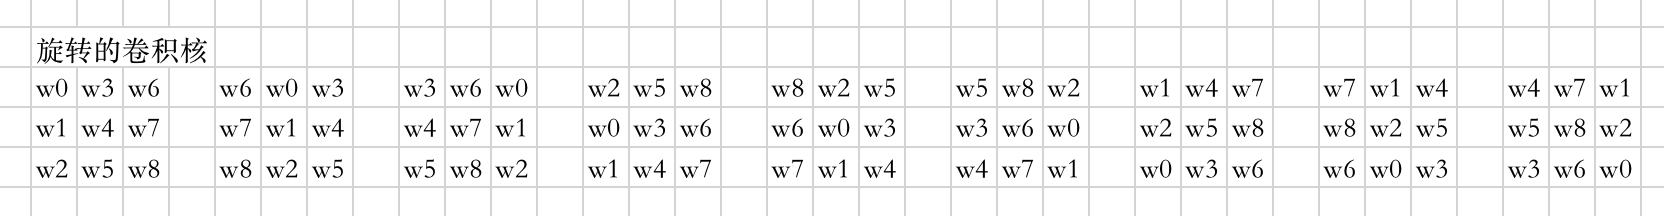
\includegraphics[width=12cm,height=1.8cm]{figures/rotated_kernel.png}
    \caption{输入和卷积核}
    \label{fig:rotated_kernel}
\end{figure} 

多路复用器对应卷积核选取输入数据的排序如下图\ref{fig:multiplexor}所示。
\begin{figure}[htbp]
    \centering
    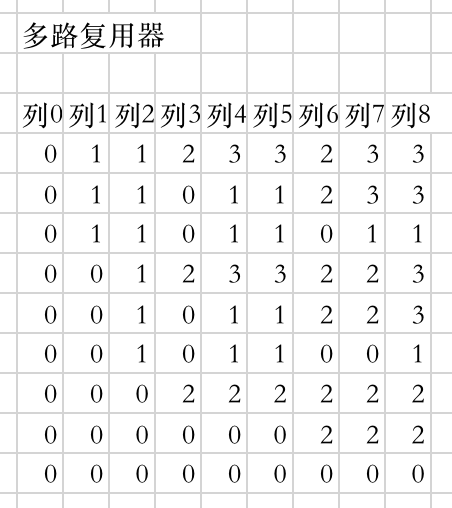
\includegraphics[]{figures/multiplexor.png}
    \caption{输入和卷积核}
    \label{fig:multiplexor}
\end{figure} 

在脉动阵列运行时,模块中的脉动数据配置子模块会根据向量输入队列和多路复用器来依次输入数据到脉动阵列中。
下面图\ref{fig:systolic_data_col0}和图\ref{fig:systolic_data_col4}分别是多路复用器选择的第一组数据和第四组数据。
激活输入矩阵按照卷积核的大小,切割成四组数据,分别按四路放置于向量输入队列中。
多路复用器中的编码就是指的向量输入队列的编号。
可以推论,向量输入会按照脉动的频率向脉动阵列中输入数据,在输入时使用多路复用器来选择使用哪一路的数据。
\begin{figure}[htbp]
    \centering
    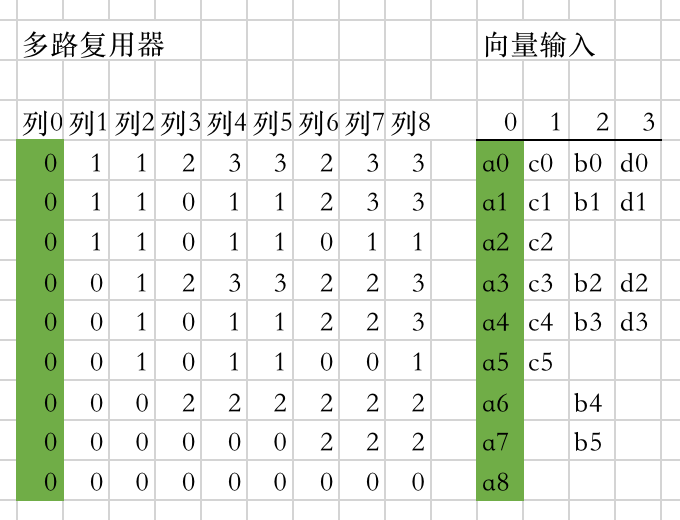
\includegraphics[width=12cm]{figures/systolic_data_col0.png}
    \caption{多路复用器选择第0列数据}
    \label{fig:systolic_data_col0}
\end{figure} 

\begin{figure}[htbp]
    \centering
    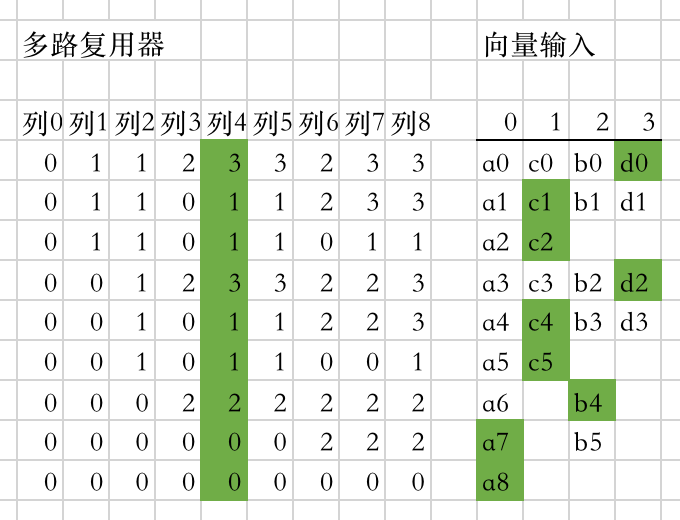
\includegraphics[width=12cm]{figures/systolic_data_col4.png}
    \caption{多路复用器选择第4列数据}
    \label{fig:systolic_data_col4}
\end{figure} 
当输入数据和权重都放到指定的运算单元后,脉动阵列会执行乘法和累加运算。
以此可见,脉动阵列向下传递的是向量输入和部分和。
最终在输入脉动阵列的数据全都经过计算之后,得到输出的值。
详细的完整例子,可见附录B。



\subsection{建模与IC验证}
在IC设计行业,ASIC项目的拖期情况非常严重,其中有些项目会拖期半年以上。
除了项目容易延期,ASIC项目的失败率也非常高。
小米的澎湃S2处理器曾多次流片失败。
研发一款ASIC芯片的道路充满了艰难险阻。
ASIC芯片的特点与简单指令集的CPU完全相反,它被设计出来的目的就是为了实现复杂功能。
所以ASIC芯片的设计一般都是以具体业务作为需求。
这会导致其设计过程非常繁琐。
如图\ref{fig:asic_flow}是ASIC的开发流程图.IC设计公司会在项目初始时完成市场需求设计(MRD)和产品需求设计(PRD)。
\begin{figure}[htbp]
    \centering
    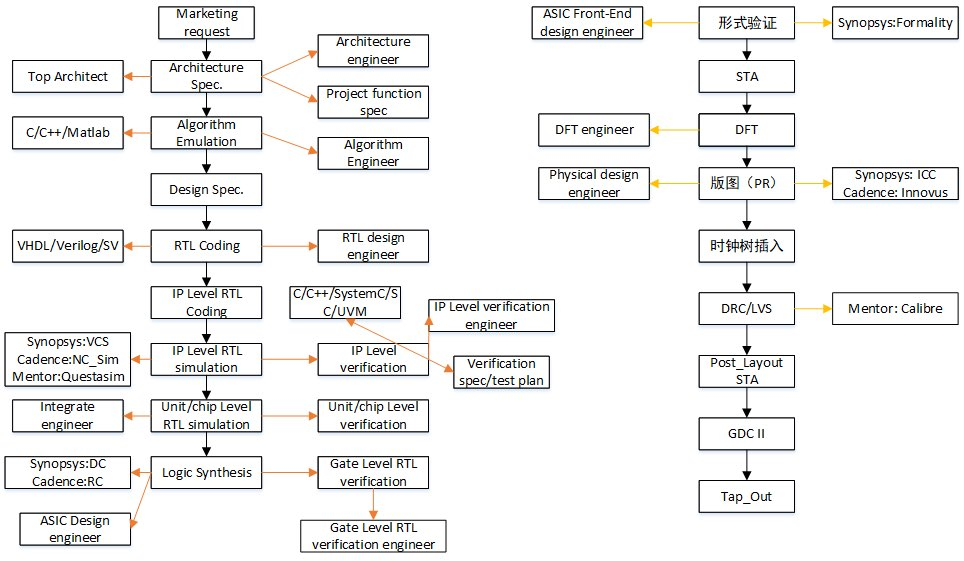
\includegraphics[width=12cm,height=7cm]{figures/asic_flow.jpeg}
    \caption{ASIC开发流程图}
    \label{fig:asic_flow}
\end{figure}
在需求被明确之后,系统工程师就会开始进行架构设计。
这个过程包含了提出顶层架构设计和定义需求中所有用例涉及到的子模块,并且定义各个子模块之间的连接关系、交互方式和时序要求。
在完成芯片的架构设计之后,需要对芯片进行建模。芯片建模是用一种高级语言对芯片的行为进行描述。
一般会采用C/C++或者SystemC来实现建模。
如果涉及到新的算法模块,会要求算法工程师先做出算法的Matlab或者C模型,作为模块开发者和芯片模型的参考依据。   

% 简述IC验证
芯片在流片之前,需要进行完整和详细的IC验证工作。
工程师需要尽可能地找出项目的缺陷,从而降低流片的风险,节省人力和物力资源。
% 简述什么是建模
芯片建模是用一种高级语言对芯片的行为进行描述,常用的高级语言有C/C++或System C。
% 为什么使用python和C/C++建模
使用C-Model进行建模和仿效,是一种低成本且有效的模块级验证方法。
而使用python可以更快速地对算法建模。
在ASIC项目越来越复杂的今天,使用C/C++或者python进行建模来验证算法是保障项目质量的重要手段。
在IC设计公司中,使用软件建模、软件仿真和FPGA仿真都是常见的仿效或者仿真的方法。
C/C++或python建模可以视为仅需要人力成本。
其编码所需的时间较长,而编译所需的时间和仿真所需的时间都很短。
软件仿真的成本在于仿真软件的授权,其编码的规模一般比编写C/C++或python软件的规模小,但它的缺点是仿真所花费的时间非常长。
FPGA设备非常昂贵单台设备的价值可能是数万至数十万元人民币,其编码和仿真所需的时间不多,但其编译所需的时间非常长。
编译一个可烧录的文件经常需要数小时甚至数十小时。

\paragraph{SystemC}
在建模的过程中将会采用SystemC作为建模的语言。
SystemC既是系统级语言,也是硬件描述语言\cite{2008SystemC}。
%引用《SystemC入门》(第二版)
SystemC 由 C++发展而来,是优秀的系统级描述语言,SystemC 单元库结构如图\ref{fig:systemc_libs}所示,它使软硬件工程师可以在统一的环境下同时描述软硬件结构和接口, 它将通信与功能分开,能提供更高设计效率,将集成电路设计引入事务级,提供 更有效的设计流程,从而帮助解决集成电路产业面临的各种问题,从此可以预见 SystemC 的光明前景\cite{SWZ20131553B}。
% 引用 单中伟. 1553B 总线远程终端的 FPGA 程序设计[J]. 现代电子技术, 2013(09): 28-30.

\begin{figure}[htbp]
    \centering
    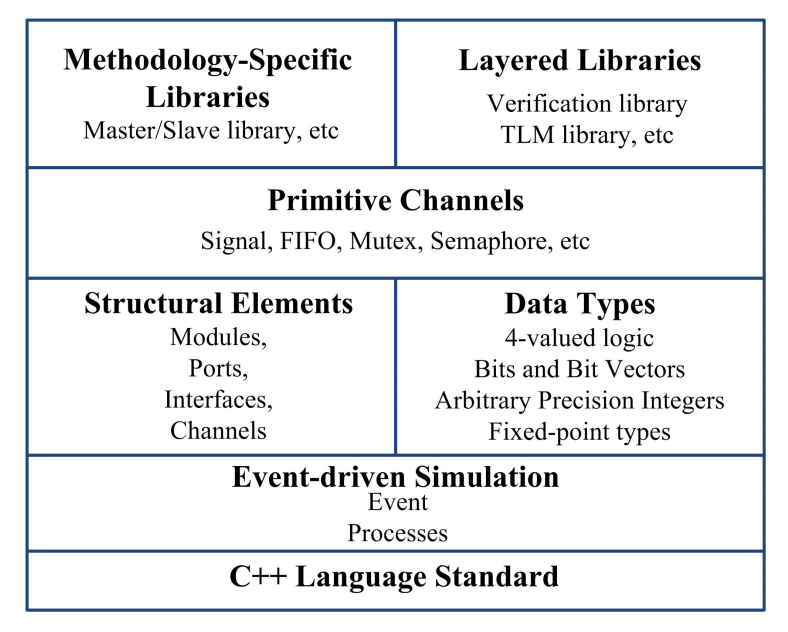
\includegraphics[width=8cm]{figures/systemc_libs.png}
    \caption{SystemC单元库}
    \label{fig:systemc_libs}
\end{figure} 
传统的硬件设计使用如 Verilog HDL 或者 VHDL 等硬 件描述语言,而软件设计则使用不同的语言,所以在进行软硬件协同验证时比较 困难,并且软件的设计往往要迟于硬件系统证成为制约设计效率的主要因素为提高 工作效率,人们引进了 SystemC 语言,使得在运用 SystemC 对硬件进行建模时, 可以在一开始就能够同时进行软硬件的设计,这是传统的 SoC 设计所比不了的\cite{2010Real}。
%引用 Zhao Changyu, Yan Changxiang, Yu Ping. Real time scheduling of messages on 1553B bus[J]. Optics and Precision Engineering, 2010, 18(3): 732-40.
在下文的“建模和验证”章节,将使用SystemC作为实现本文设计的建模语言,实现系统级建模和算法的仿效。

\section{主要研究内容和意义}

%TODO CIS增强芯片	神经网络推理 系统级建模
%TODO 研究一种CIS片内的神经网络推理模块的系统级建模
本课题的主要工作内容就是在良好的理解计算机系统,以及对深度学习神经网络算法有一定理解的基础上,运用系统级建模的方法,设计和建模一种能够加速CIS芯片片内进行深度学习神经网络推理运算的方案。  
本课题设计的CIS深度学习神经网络运算加速方案,实现了一种基于脉动阵列的ResNet18的神经网络来进行推理。
其整体结构是基于当前比较先进的堆栈式CIS芯片,在CIS片内集成了传感器核心、深度学习神经网络运算模块以及其他的功能模块。
在设计深度学习神经网络加速器时,本文将讨论和设计脉动阵列的设计,以及神经网络算法在脉动阵列上的应用。    


这种设计实践了“软件定义硬件”的新概念。
其设计和建模过程本身就是一种方法学的探索。
在进行芯片的设计时,系统级建模和算法验证是其中的关键部分。
本文通过构建CIS芯片上的深度学习神经网络加速器的系统级模型,将需要处理的诸多硬件信号作为抽象数据类型进行操作,忽略RTL管脚的通信细节,通过调用相应函数来进行模块之间的通信,提高仿真的速度\cite{2007ESL}。
%引用  Weijers J.W, Glassee M, Schuster T. ESL design and HW/SW co-verification of high-end Software Defined Radio platforms[C]. Hardware/Software Codesign and System Synthesis (CODES+ISSS), 2007 5th IEEE/ACM/IFIP International Conference, Salzburg, 2007: 191-196.
在充分描述系统控制逻辑和算法后,通过SystemC来实现建模的工作。

% !TEX root = ../main.tex

\chapter{架构与模块设计}

\section{总体架构设计}

从图<Figure 1>中可以看到这是经典的图像传感器与ISP(Image Sensor Processor)以及其他功能部件连接在一条高速数据总线的结构。
总体架构可以分为几个部分:数据通路部分、系统控制部分和高速数据总线。
数据通路部分包含了IDA(Input Data Adapter)、深度学习神经网络加速模块、TX输出模块。
系统控制部分包含了CPU、DMA、Memory、SPI Flash以及其他外设模块(比如I2C和UART等接口模块)。
%TODO 架构图展示
\begin{figure}[htbp]
    \centering
    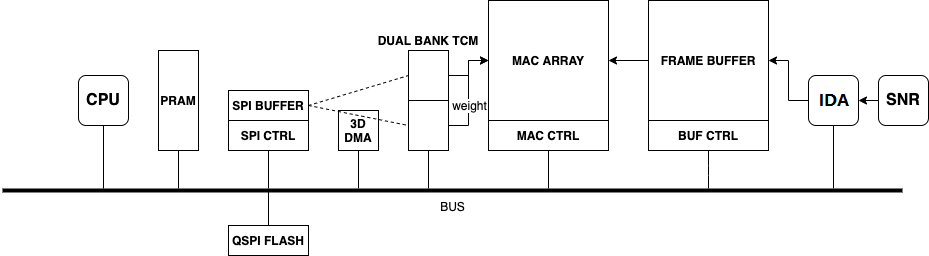
\includegraphics[width=15cm,height=4.5cm]{figures/bnn.png}
    \caption{总体架构图}
    \label{1}
\end{figure}
%TODO 各个模块的简述
在设计和建模过程中,假设从ISP输出的数据为我们人体肉眼可见的视频数据流。
为了减少建模过程中的非相关设计,这里的视频数据流假设为RGB888的格式。

\section{CIS数据通路}
%TODO 展示Stream datapath的传输方式 sof eof href
%TODO DL accelerator在数据通路中的作用
%TODO Fix Timing模块做数据同步,最后输出结果
CIS芯片的作用,就是将图像传感器接收到的信号,转为数字信号后传输给后端。一般来说,我们把CIS
芯片上的设计逻辑称为数据通路。图像数据通路一般由输入、数据处理和输出三个部分组成。通常地,这三个部分也具有各自不同的时钟域。
在输入时钟域中,RX模块接收从CMOS传感器输出的数据。由IDA模块的缓冲区暂存数据后向后一个时钟域输出同步数据。
在数据处理的时钟域中,深度学习运算模块将进行推理操作。
在输出时钟域中,FT(fix timing)模块将调整输出的时钟频率.TX模块负责以指定格式输出图像数据。  

\subsection{数据流的输入}
%TODO 
%   数据流的输入将由IDA(Input Data Adapter)模块处理。这个模块的主要作用是将Sensor输出的数据放到一个缓存区。
%   并将视频数据流的plck同步到数据流的时钟域。

这里假设从图像传感器输出的图像数据为224x224像素尺寸的图像。
视频数据流的输入需要参考流式设备的特性,合理的缓存大小和同步的时机是关键点。
对于卷积运算,缓存的行数大小应该大于等于卷积核的行数和列数之间的较大值。
例如,卷积核的尺寸为3x3时,缓存至少要保存3行数据。
如果,每帧图像的尺寸为224x224个像素点。
由RGB三个通道组成的每一帧都拆分成三个224x224x8比特。
那么需要给一个通道的一帧数据缓存的大小需要大于等于672个字节。


\subsection{数据流中的运算}
% TODO
% 在数据流中实时运算图像识别的算法

在数据通路中实时地进行图像识别的运算,是本设计的核心思想。
运算的模块将通过帧同步信号和行同步信号等机制来处理缓存的数据。
在实际应用时,将用于图像识别的人工智能处理器在物理位置上比较靠近图像来源(CMOS/CCD传感器),这样就避免了图像数据需要DRAM的存储。
另外,对于CNN算法,其中常用的一类CNN是共享权值的,这样权值的数量就不大,可以完整存放在片上SRAM中,从而使得权值也能避免存储在DRAM中。
这样处理后,整个系统就不需要DRAM做存储,从而大幅降低功耗。
设计3个缓存分别用于存储权值、输入数据、输出数据。
核心的运算模块是由最小运算单元组成的运算单元阵列。
普通的运算阵列受限于其规模。它的规模越大,需要的传输布线长度约长,传输时间越久,因此频率也无法做到很高。
这样的话,它的运算性能就会受到规模大小的限制。  
\begin{figure}[htbp]
    \centering
    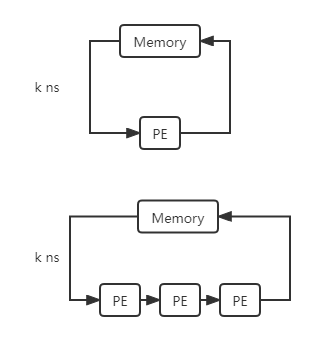
\includegraphics[]{figures/systolic_array.png}
    \caption{脉动阵列原理图}
    \label{systolic}
\end{figure}

如果采用脉动阵列,那么就能避免这种问题。
脉动一词原本是来自心血管。
在冯诺依曼的计算机体系中,指令和数据是一起存储在存储器中。
在运算的过程中,数据从存储器中被取出,经过处理器的处理后再写回到存储器中。
这个过程就像是人体的血液循环一样,因此得名脉动。
当运算的过程是由多个可重复的运算单元组成时,每一个运算单元都会与一个或者多个周围的单元发生数据交互,结果或将存储在运算单元内部,或将传递给下一个单元。
在脉动阵列中,最重要的是设计一种在运算单元之间联系的规则,并且把高层次的算法映射到每一个单元上。
脉动阵列的优势如图2-2所示,在某种计算需要计算单元迭代执行3次时,可以减少(3-1)次的存储器读写时间。
这里的脉动阵列是使用乘累加器作为其处理单元的。
它非常适合如矩阵运算,卷积等等数据流具有一定规律的算法。


\section{深度学习神经网络运算单元}

% TODO CPU和GPU平台上的加速运算
在常见的CPU和GPU平台上,SIMT和SIMD等技术被广泛地应用。
从字面上解释,SIMT是单指令多线程,而SIMD为单指令多数据流。
在SIMD中,向量中的元素处在相同的地址空间。
而SIMT中的每一个线程的寄存器都是私有的。可以通过共享内存或是其他的线程内同步机制来进行通信。


\subsection{影响因子和依据}
在开始设计深度学习神经网络的运算模块之前,本章节将提出一些影响设计的因素,并描述如何将这些因素考虑在内来帮助我们完成设计。
其中精准度、吞吐量、延迟、能效比和功耗,都是衡量深度学习神经网络运算的硬件单元的最重要因素。


% TODO 精确度 吞吐量和延迟 能效比和功耗
准确度是这类问题中最常见的一个指标。对于图像分类问题,准确度报告为正确分类图像的百分比,而对于目标检测问题,精度报告为平均准确度。
影响准确性的因素包括任务的难度和数据集。因此,准确度在建模的过程中将被用来验证设计的正确性。
吞吐量用于指示在给定时间段内可以处理的数据量或可以完成的任务的执行次数。高吞吐量通常是应用程序的关键。
延迟度量输入数据到达系统和生成结果之间的时间。低延迟对于实时交互应用程序(如虚拟现实、自主导航和机器人技术)是必要的。
吞吐量和延迟通常被认为是可以直接相互派生的。
一般的,在给定能量单位下可处理的数据量或完成任务的执行次数被称为能效比。




\subsection{基于脉动阵列的深度残差网络}
本文中将基于脉动阵列来实现深度残差网络。

%TODO ResNet18的Basic Block
%TODO x -> conv3x3 -> BN -> Relu -> conv3x3 -> BN ( + 入口的x)-> out -> Relu -> out
%TODO x -> conv7x7,stride=3,padding=3 -> BN -> 



%TODO 脉动阵列实现矩阵乘法的CMODEL
脉动阵列是1978年KUNG H T提出的一种应用在片上多处理器的体系结构。它是由多个相同的、结构简单的计算单元
以网状形式连接而成的,具有并行性、规律性和局部通信的特征。在深度残差网络ResNet18中,由5个卷积层组成,
除了第一个卷积层外,后4个卷积层都是由2个基础块组成。基础块的结构如下图x所示。其中的批量标准化和Relu函
数都可以设计专用的运算模块,而3x3的卷积运算可以通过脉动阵列来运算。


%REF KUNG H T, Leiserson C E. Systolic arrays(for VLSI)[C]. Sparse Matrix Proceedings 1978, Society for Industrial and Applied Mathematics, 1979.

脉动阵列的设计和C模型实现,可以分为两个部分:脉动阵列模块的顶层设计和处理单元的设计。
处理单元(PE)的寄存器:时钟、重置、同步清零、输入参数A、输入参数B、输出给下一级的A、输出给下一级的
B、输出P值。

\begin{table}[!hpt]
    \bicaption[PE的寄存器表]{PE的寄存器表}{Register Table Of PE}
    \label{tab:firstone}
    \centering
    \begin{tabular}{@{}lllr@{}} \toprule
        Type & Name & Description & Size \\ \midrule
        input  & CLK  & 输入PE模块的时钟信号 & 32b \\
        input  & RST  & 模块重置寄存器 & 16b \\
        input   & SCLR   & 同步清零寄存器 & 16b \\
        input   & A   & 输入参数A & 8b \\
        input   & B   & 输入参数B & 8b \\
        output   & Next\_A   & 输出到下一个PE的A & 8b \\
        output   & Next\_B   & 输出到下一个PE的B & 8b \\
        output & P & PE的运算结果P & 16b \\ \bottomrule
    \end{tabular}
  \end{table}

  

% \begin{table}[!hpt]
%     \caption[PE的寄存器表]{PE的寄存器表}{Register Table Of PE}
%     \label{tab:firstone}
%     \centering
%     \begin{tabular}Type & Name & Description & Size \\  \toprule
%       input & CLK  & 输入PE模块的时钟信号 & 32b \\ \midrule
%       input & RST  & 模块重置寄存器 & 16b \\
%       input & SCLR & 同步清零寄存器 & 16b \\
%       input & A & 输入参数A & 8b \\
%       input & B & 输入参数B & 8b \\
%       output & Next_A & 输出到下一个PE的A & 8b \\
%       output & Next_B & 输出到下一个PE的B & 8b \\
%       output & P & PE的运算结果P & 16b \\ \bottomrule
%     \end{tabular}
% \end{table}  



\section{存储}
%TODO 关于存储Multiple Bank的设计(状态机)
本设计中,专门对存储进行了优化,区分开了不同的RAM区域来存储不用的数据,主要由以下几个区域:存储输入和输出数据的
INRAM和OUTRAM、存储网络数据的NRAM、存储权重的WRAM、存储系统数据的SRAM以及存储临时数据的TRAM。拆分存储的设计
主要有以下两大好处:读写的带宽和避免冲突。
拆分存储之后,SRAM可以被调整为适当的读写宽度。假设输入和输出的宽度是$X_a \times K$字节,存储网络和权重数据的
NRAM和WRAM为$X_a \times X_a \times K$字节。如果是用CPU或GPU,且未做优化的情况下,处理器只能按照固定宽度读取
数据。

DRAM和SRAM
先进的存储技术可以降低高密度存储器(如DRAM)的访问能量。
例如,嵌入式DRAM(eDRAM)在芯片上提供高密度存储器,以避免关闭芯片电容的高能耗成本[97];eDRAM的密度比SRAM高2.85倍,能效比DRAM高321倍(DDR3)[93]。
与DRAM相比,eDRAM还提供了更高的带宽和更低的延迟。在DNN处理中,eDRAM可用于在芯片上存储数十兆字节的权重和激活,以避免芯片外访问,如DaDianNao[93]所示。
eDRAM的缺点是其密度低于片外DRAM,并且会增加芯片成本。
DRAM也可以使用硅通孔(TSV)堆叠在芯片顶部,而不是将DRAM集成到芯片本身。
这项技术通常被称为三维存储器,并已以混合存储立方体(HMC)[98]和高带宽存储器(HBM)[99]的形式商业化。
3-D内存提供了一个数量级的更高带宽,并且相对于现有的2-D DRAM,访问能量减少了5倍,因为TSV的电容低于典型的片外互连。
最近的工作探索了使用HMC以多种方式高效处理DNN。例如,Neurocube[100]将SIMD处理器集成到HMC的逻辑芯片中,使内存和计算更紧密地结合在一起。
Tetris[101]探讨了HMC与Eyeris空间架构和行固定数据流的结合使用。
它建议分配比片上存储器更多的计算区域(即更大的PE阵列和更小的全局缓冲区),以利用HMC的低能量和高吞吐量特性。它还调整数据流,以考虑HMC内存和更小的片上内存。
Tetris在使用传统2-D DRAM的基线系统上实现了1.5倍的能耗降低和4.1倍的吞吐量增加。

SRAM不是将内存放在计算附近,而是将计算放在内存中。
例如,乘法和累积操作可以直接集成到SRAM阵列的位单元中[102],如图36(a)所示。
在这项工作中,使用5位DAC将字线(WL)驱动到表示特征向量的模拟电压,而位单元存储二进制权重±1。
比特单元电流(IBC)实际上是特征向量的值和存储在比特单元中的权重的值的乘积;来自列中位单元的电流加在一起对位线(VBL)放电。
与从SRAM读取1位权重并单独执行计算相比,该方法可节省12倍的能量。
为了对抗电路的非理想性,DAC考虑了关于WL电压的非线性位线放电,并使用升压来组合易受设备变化影响的弱分类器,以形成强分类器[103]。

非易失性电阻存储器
乘法和累积操作也可以直接集成到高级非易失性高密度存储器中,方法是将其用作可编程电阻元件,通常称为忆阻器[105]。
具体地,如图36(b)所示,以电阻器的电导作为权重,以电压作为输入,以电流作为输出,执行乘法。
加法是通过将不同忆阻器的电流与基尔霍夫电流定律相加来完成的。这是权重固定数据流的最终形式,因为权重始终保持在适当的位置。
这种方法的优点包括:由于计算被嵌入内存中,从而减少了数据移动,因此降低了能耗;由于内存和计算可以以与DRAM类似的密度进行密集封装,因此增加了密度[106]。
非易失性电阻存储器器件有几种常见的候选器件,包括相变存储器(PCM)、电阻RAM(RRAM或ReRAM)、导电桥RAM(CBRAM)和自旋转移转矩磁RAM(STT-MRAM)[107]。
这些设备在耐久性(即可以写入多少次)、保留时间、写入电流、密度(即单元大小)、变化和速度方面有不同的权衡。
如[108]所述,使用非易失性电阻存储器进行处理有几个缺点。
首先,它受到前面描述的模拟处理的精度降低和ADC/DAC开销的影响。
第二,阵列尺寸受到连接电阻器件的导线的限制;具体而言,对于大型阵列(例如1k×1k),导线能量占主导地位,并且沿导线的红外压降会降低读取精度。
第三,对电阻器件进行编程的写入能量可能非常昂贵,在某些情况下需要多个脉冲。
最后,电阻器件还可能受到器件间和周期间变化的影响,在整个电导范围内具有非线性电导。



% !TeX root = ../main.tex

\chapter{建模与验证}

% TODO 解释C模型在ASIC设计中的作用                                          
据统计,全世界有67\%以上的ASIC项目都是拖期交付的,其中有些项目会拖期半年以上,从这个数据可以想象得到,通向一款ASIC芯片的道路会有多么曲折。
ASIC芯片的特点与简单指令集的CPU完全相反,它被设计出来的目的就是为了实现复杂功能。
因此,ASIC芯片的设计过程异常繁琐。
一般的,芯片公司会在项目初始时,完成市场需求设计和产品需求设计。
在需求被明确之后,系统工程师就会开始进行架构设计。
这个过程包含了提出顶层架构设计和定义需求中所有用例涉及到的子模块。
并且,定义各个子模块之间的连接关系、交互方式和时序要求。
在完成芯片的架构设计之后,需要对芯片进行建模。芯片建模是用一种高级语言对芯片的行为进行描述。
一般会采用C/C++或者SystemC来实现建模。
如果涉及到新的算法模块,会要求算法工程师先做出算法的Matlab或者C模型,作为模块开发者和芯片模型的参考依据。

\section{顶层架构}
在章节2.1中,本文已经简述了总体的架构设计。本章节将详细说明顶层架构的C模型。


\section{数据的输入}
需要设计相应的模块处理输入的图像数据,使得神经网络计算模块可以进行计算。
%TODO 描述DVP并口传输input的数据
%DRAFT 设计有下列端口
%       PCLK        像素点同步时钟信号
%       XCLK        外部输入时钟信号
%       VSYNC       帧同步信号
%       HSYNC       行同步信号
%       Data[0:11]  数据信号12bit


%TODO 设计Input Data Adapter
%       buffer      5行buffer


\section{数据的运算}  

\subsection{脉动阵列的仿真}
% TODO 首先实现脉动和PE
定义处理单元和实现脉动的行为。
\begin{codeblock}[language=C]
#include <iostream>
#include <cstdlib>
#include <ctime>
#include <iomanip>
#define N 256
using namespace std;

typedef struct PE{
    int weight;
    int neuron;
    int psum;
};

class Systolic{
public:
    PE S[N][N];
public:
    void Init(){
        for(int i=0;i<N;i++)
            for(int j=0;j<N;j++){
                S[i][j].psum=0;
                S[i][j].weight=0;
                S[i][j].neuron=0;
            }
    }
    void calc(){
        for(int i=0;i<N;i++)
            for(int j=0;j<N;j++)
                S[i][j].psum+=S[i][j].weight*S[i][j].neuron;
    }
    void shift(int a[N],int b[N]){
        //水平方向传播矩阵A,a[N]是本次要被读入的列(left->right)
        for(int i=0;i<N;i++)
            for(int j=N-1;j>0;j--){
                S[i][j].neuron=S[i][j-1].neuron;
        }
        for(int i=0;i<N;i++)
            S[i][0].neuron=a[i];
        //竖直方向上传播矩阵B,b[N]是本次要被读入的行(up->bottom)
        for(int j=0;j<N;j++)
            for(int i=N-1;i>0;i--){
                S[i][j].weight=S[i-1][j].weight;
        }
        for(int j=0;j<N;j++)
            S[0][j].weight=b[j];
    }
    void Display(){
        cout<<"weight:"<<endl;
        for(int i=0;i<N;i++){
            for(int j=0;j<N;j++)
                cout<<fixed<<setw(4)<<S[i][j].weight<<",";
            cout<<endl;
        }
        cout<<"neuron:"<<endl;
        for(int i=0;i<N;i++){
            for(int j=0;j<N;j++)
                cout<<fixed<<setw(4)<<S[i][j].neuron<<",";
            cout<<endl;
        }
    }
};

\end{codeblock}




% !TEX root = ../main.tex

\chapter{结果与报告}

\section{测试用例}

\subsection{算法的可行性}



\subsection{空间占用和并行性}



\section{报告}

按照教务处的要求,参考文献外观应符合国标 GB/T 7714 的要求。模版使用 \BibLaTeX\
配合 \pkg{biblatex-gb7714-2015} 样式包
\footnote{\url{https://www.ctan.org/pkg/biblatex-gb7714-2015}}
控制参考文献的输出样式,后端采用 \pkg{biber} 管理文献。

请注意 \pkg{biblatex-gb7714-2015} 宏包 2016 年 9 月才加入 CTAN,如果你使用的
\TeX\ 系统版本较旧,可能没有包含 \pkg{biblatex-gb7714-2015} 宏包,需要手动安装。
\BibLaTeX\ 与 \pkg{biblatex-gb7714-2015} 目前在活跃地更新,为避免一些兼容性问
题,推荐使用较新的版本。

正文中引用参考文献时,使用 \verb|\cite{key1,key2,key3...}| 可以产生“上标引用的
参考文献”,如 \cite{Meta_CN,chen2007act,DPMG}。使用
\verb|\parencite{key1,key2,key3...}| 则可以产生水平引用的参考文献,例如
\parencite{JohnD,zhubajie,IEEE-1363}。请看下面的例子,将会穿插使用水平的和上标的
参考文献:关于书的\parencite{Meta_CN,JohnD,IEEE-1363},关于期刊的
\cite{chen2007act,chen2007ewi},会议论文 \parencite{DPMG,kocher99,cnproceed},硕
士学位论文\parencite{zhubajie,metamori2004},博士学位论文
\cite{shaheshang,FistSystem01,bai2008},标准文件 \parencite{IEEE-1363},技术报告
\cite{NPB2},电子文献 \parencite{xiaoyu2001, CHRISTINE1998},用户手册
\parencite{RManual}。

可以使用 \verb|\nocite{key1,key2,key3...}| 将参考文献条目加入到文献表中但不在正
文中引用。使用 \verb|\nocite{*}| 可以将参考文献数据库中的所有条目加入到文献表
中。

% !TEX root = ../main.tex

\begin{summary}
这里是全文总结内容。

本课题阐述了一种CIS芯片上的深度学习神经网络加速器的设计方案,并建模进行了算法级的验证。
%总结一下设计
该设计利用了图像传感器中流水线式的数据通路的特性,将神经网络加速器设置在数据通路中。
这样的设计避免了运算时对低速存储设备(例如DRAM)的读写,来提升神经网络算法的运算速度。
同时,采用了脉动阵列来做神经网络算法中的乘加运算。
巧合的是,脉动阵列的特性也与图像传感器的数据通路特性一致。  
因此,无论从节省存储设备空间的角度,还是从并行执行算法节省时间的角度来说,这种设计都是优于CIS芯片外进行图像识别的方案的。  

近年,“感知时代”的概念兴起。传感器与人工智能的结合正在给人类带来新的技术革新。
同时,随着摩尔定律的失效,体系结构的变革带来了“异构计算”。
而本课题的研究内容正是“感知”加上“异构”的王炸组合。
AI芯片初创公司Groq提出了“软件定义硬件”。
这种说法在业界看来虽然为时尚早,但我们也可以从中看到,在追求极致性能的产品上,被开发的远不只是软件,硬件也是需要重新定义的。


\end{summary}


%TC:ignore

% 使用英文字母对附录编号
\appendix

% 附录内容
% !TEX root = ../main.tex

\chapter{Maxwell Equations}

选择二维情况,有如下的偏振矢量:
\begin{subequations}
  \begin{align}
    {\bf E} &= E_z(r, \theta) \hat{\bf z}, \\
    {\bf H} &= H_r(r, \theta) \hat{\bf r} + H_\theta(r, \theta) \hat{\bm\theta}.
  \end{align}
\end{subequations}
对上式求旋度:
\begin{subequations}
  \begin{align}
    \nabla \times {\bf E} &= \frac{1}{r} \frac{\partial E_z}{\partial\theta}
      \hat{\bf r} - \frac{\partial E_z}{\partial r} \hat{\bm\theta}, \\
    \nabla \times {\bf H} &= \left[\frac{1}{r} \frac{\partial}{\partial r}
      (r H_\theta) - \frac{1}{r} \frac{\partial H_r}{\partial\theta} \right]
      \hat{\bf z}.
  \end{align}
\end{subequations}
因为在柱坐标系下,$\overline{\overline\mu}$ 是对角的,所以 Maxwell 方程组中电场
$\bf E$ 的旋度:
\begin{subequations}
  \begin{align}
    & \nabla \times {\bf E} = \upi \omega {\bf B}, \\
    & \frac{1}{r} \frac{\partial E_z}{\partial\theta} \hat{\bf r} -
      \frac{\partial E_z}{\partial r}\hat{\bm\theta} = \upi \omega \mu_r H_r
      \hat{\bf r} + \upi \omega \mu_\theta H_\theta \hat{\bm\theta}.
  \end{align}
\end{subequations}
所以 $\bf H$ 的各个分量可以写为:
\begin{subequations}
  \begin{align}
    H_r &= \frac{1}{\upi \omega \mu_r} \frac{1}{r}
      \frac{\partial E_z}{\partial\theta}, \\
    H_\theta &= -\frac{1}{\upi \omega \mu_\theta}
      \frac{\partial E_z}{\partial r}.
  \end{align}
\end{subequations}
同样地,在柱坐标系下,$\overline{\overline\epsilon}$ 是对角的,所以 Maxwell 方程
组中磁场 $\bf H$ 的旋度:
\begin{subequations}
  \begin{align}
    & \nabla \times {\bf H} = -\upi \omega {\bf D}, \\
    & \left[\frac{1}{r} \frac{\partial}{\partial r}(r H_\theta) - \frac{1}{r}
      \frac{\partial H_r}{\partial\theta} \right] \hat{\bf z} = -\upi \omega
      {\overline{\overline\epsilon}} {\bf E} = -\upi \omega \epsilon_z E_z
      \hat{\bf z}, \\
    & \frac{1}{r} \frac{\partial}{\partial r}(r H_\theta) - \frac{1}{r}
      \frac{\partial H_r}{\partial\theta} = -\upi \omega \epsilon_z E_z.
  \end{align}
\end{subequations}
由此我们可以得到关于 $E_z$ 的波函数方程:
\begin{equation}
  \frac{1}{\mu_\theta \epsilon_z} \frac{1}{r} \frac{\partial}{\partial r}
  \left(r \frac{\partial E_z}{\partial r} \right) + \frac{1}{\mu_r \epsilon_z}
  \frac{1}{r^2} \frac{\partial^2E_z}{\partial\theta^2} +\omega^2 E_z = 0.
\end{equation}

% !TEX root = ../main.tex

\chapter{绘制流程图}

图~\ref{fig:flow_chart} 是一张流程图示意。使用 \pkg{tikz} 环境,搭配四种预定义节
点(\verb+startstop+、\verb+process+、\verb+decision+和\verb+io+),可以容易地绘
制出流程图。

\begin{figure}[!htp]
  \centering
  \resizebox{6cm}{!}{\begin{tikzpicture}[node distance=2cm]
    \node (pic) [startstop] {待测图片};
    \node (bg) [io, below of=pic] {读取背景};
    \node (pair) [process, below of=bg] {匹配特征点对};
    \node (threshold) [decision, below of=pair, yshift=-0.5cm] {多于阈值};
    \node (clear) [decision, right of=threshold, xshift=3cm] {清晰?};
    \node (capture) [process, right of=pair, xshift=3cm, yshift=0.5cm] {重采};
    \node (matrix_p) [process, below of=threshold, yshift=-0.8cm] {透视变换矩阵};
    \node (matrix_a) [process, right of=matrix_p, xshift=3cm] {仿射变换矩阵};
    \node (reg) [process, below of=matrix_p] {图像修正};
    \node (return) [startstop, below of=reg] {配准结果};
     
    %连接具体形状
    \draw [arrow](pic) -- (bg);
    \draw [arrow](bg) -- (pair);
    \draw [arrow](pair) -- (threshold);

    \draw [arrow](threshold) -- node[anchor=south] {否} (clear);

    \draw [arrow](clear) -- node[anchor=west] {否} (capture);
    \draw [arrow](capture) |- (pic);
    \draw [arrow](clear) -- node[anchor=west] {是} (matrix_a);
    \draw [arrow](matrix_a) |- (reg);

    \draw [arrow](threshold) -- node[anchor=east] {是} (matrix_p);
    \draw [arrow](matrix_p) -- (reg);
    \draw [arrow](reg) -- (return);
\end{tikzpicture}
}
  \bicaption{绘制流程图效果}{Flow chart}
  \label{fig:flow_chart}
\end{figure}


% 后文部分无编号
\backmatter

% 参考文献
\printbibliography[heading=bibintoc]

% 用于盲审的论文需隐去致谢、发表论文、科研成果、简历

% 致谢
% !TEX root = ../main.tex

\begin{acknowledgements}
  感谢张忠能老师
  感谢姚天昉老师
\end{acknowledgements}


% 发表论文、科研成果、简历
% 盲审论文中,发表论文及科研成果等仅以第几作者注明即可,不要出现作者或他人姓名
% !TEX root = ../main.tex

\begin{publications}
  \item Chen H, Chan C~T. Acoustic cloaking in three dimensions using acoustic metamaterials[J]. Applied Physics Letters, 2007, 91:183518.
  \item Chen H, Wu B~I, Zhang B, et al. Electromagnetic Wave Interactions with a Metamaterial Cloak[J]. Physical Review Letters, 2007, 99(6):63903.
\end{publications}

\begin{publications*}
  \item 第一作者. 中文核心期刊论文, 2007.
  \item 第一作者. EI 国际会议论文, 2006.
\end{publications*}

% % !TEX root = ../main.tex

\begin{achievements}
  \item 第一发明人,“永动机”,专利申请号202510149890.0
\end{achievements}

\begin{achievements*}
  \item 第一发明人,“永动机”,专利申请号XXXXXXXXXXXX.X
\end{achievements*}

% !TEX root = ../main.tex

\begin{resume}
  \subsection*{基本情况}
    龚烽,1988 年 2 月生于 上海。

  \subsection*{教育背景}
  \begin{itemize}
    \item 2006 年 9 月至 2010 年 3 月,上海大学,本科,计算机科学与技术 专业
  \end{itemize}

  \subsection*{研究兴趣}
    \LaTeX{} 
    我平时的工作是一名IC设计公司的固件工程师。
    我的本职工作是芯片的验证和固件的开发。
    我研究的兴趣领域主要在嵌入式开发软硬件结合的地方。
    我比较关注半导体领域中硬件发展与市场上产品的关系。

  \subsection*{联系方式}
  \begin{itemize}
    \item 地址: 上海市浦东新区上科路 88 号,201203
    \item E-mail: \email{rick.gong@ovt.com}
  \end{itemize}
\end{resume}


% 中文学士学位论文要求在最后有一个英文大摘要,单独编页码,英文学士学位论文不需要
% % !TEX root = ../main.tex

\begin{digest}
  An imperial edict issued in 1896 by Emperor Guangxu, established Nanyang
  Public School in Shanghai. The normal school, school of foreign studies,
  middle school and a high school were established. Sheng Xuanhuai, the person
  responsible for proposing the idea to the emperor, became the first president
  and is regarded as the founder of the university.

  During the 1930s, the university gained a reputation of nurturing top
  engineers. After the foundation of People's Republic, some faculties were
  transferred to other universities. A significant amount of its faculty were
  sent in 1956, by the national government, to Xi'an to help build up Xi'an Jiao
  Tong University in western China. Afterwards, the school was officially
  renamed Shanghai Jiao Tong University.

  Since the reform and opening up policy in China, SJTU has taken the lead in
  management reform of institutions for higher education, regaining its vigor
  and vitality with an unprecedented momentum of growth. SJTU includes five
  beautiful campuses, Xuhui, Minhang, Luwan Qibao, and Fahua, taking up an area
  of about 3,225,833 m2. A number of disciplines have been advancing towards the
  top echelon internationally, and a batch of burgeoning branches of learning
  have taken an important position domestically.

  Today SJTU has 31 schools (departments), 63 undergraduate programs, 250
  masters-degree programs, 203 Ph.D. programs, 28 post-doctorate programs, and
  11 state key laboratories and national engineering research centers.

  SJTU boasts a large number of famous scientists and professors, including 35
  academics of the Academy of Sciences and Academy of Engineering, 95 accredited
  professors and chair professors of the "Cheung Kong Scholars Program" and more
  than 2,000 professors and associate professors.

  Its total enrollment of students amounts to 35,929, of which 1,564 are
  international students. There are 16,802 undergraduates, and 17,563 masters
  and Ph.D. candidates. After more than a century of operation, Jiao Tong
  University has inherited the old tradition of "high starting points, solid
  foundation, strict requirements and extensive practice." Students from SJTU
  have won top prizes in various competitions, including ACM International
  Collegiate Programming Contest, International Mathematical Contest in Modeling
  and Electronics Design Contests. Famous alumni include Jiang Zemin, Lu Dingyi,
  Ding Guangen, Wang Daohan, Qian Xuesen, Wu Wenjun, Zou Taofen, Mao Yisheng,
  Cai Er, Huang Yanpei, Shao Lizi, Wang An and many more. More than 200 of the
  academics of the Chinese Academy of Sciences and Chinese Academy of
  Engineering are alumni of Jiao Tong University.
\end{digest}


%TC:endignore

\end{document}
